\documentclass{beamer}

\usepackage[labelformat=empty]{caption}

\mode<presentation>
{
  \usetheme{Berkeley}
  \usecolortheme{seagull}
  \setbeamercovered{transparent}
}

\title{Nuclear Energy is \\ important, old, new, and complicated}
\author{Jeffrey Seifried}
\institute{Ad Delivery Team, Yelp}
\date{Advanced Learning Group, \texttt{2015-03-16}}

\AtBeginSubsection[]
{
  \begin{frame}<beamer>{Outline}
    \tableofcontents[currentsection,currentsubsection]
  \end{frame}
}


\begin{document}

\begin{frame}
  \titlepage
\end{frame}

\begin{frame}{Outline}
  \tableofcontents
\end{frame}


\section{About Me}

    \begin{frame}{I am a devout supporter of nuclear energy}

        \begin{itemize}

            \item BSNE at University of Maryland, College Park
            \begin{itemize}
                \item Became a nuclear reactor operator
                \item Spent 4 summers + 1 semester \\ at the U.S. Nuclear Regulatory Commission
            \end{itemize}

            \pause

            \item PhDNE at UC, Berkeley and Lawrence Livermore Lab
            \begin{itemize}
                \item Developed reactor simulations
                \item Propagated uncertainties through them
                \item Helped design a hybrid fusion-fission reactor
            \end{itemize}

            \pause

            \item 2 year postdoc
            \begin{itemize}
                \item Developed reactor simulations
                \item Taught a course on nuclear reactor physics
                \item Helped design a thorium-fueled breed and burn reactor
            \end{itemize}
        \end{itemize}

    \end{frame}

\section{Nuclear energy}

    \subsection{... is important}

        \begin{frame}{``Dear future generations: Please accept our apologies, we were roaring drunk on petroleum.''}{- Kurt Vonnegut}

            \begin{itemize}

                \item Coal particulates cause 10 thousand \\ deaths annually in the US
                \pause
                \item One quarter of California air pollution is from China
                \pause
                \item Climate change is just getting ramped up
                \pause

                \vspace{2em}

                \item Global energy use will increase by a third by 2040
                \pause
                \item Natural gas and oil just got a lot cheaper
                \pause
                \item Coal is and always will be cheap

            \end{itemize}

        \end{frame}

        \begin{frame}{We need a scalable, baseload, carbon-free energy source.  Right now!}

            \begin{columns}[T]

                \begin{column}{0.5\textwidth}
                    \begin{figure}
                        \centering
                        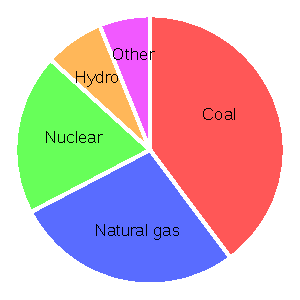
\includegraphics[width=\textwidth]{./img/sources.pdf}
                        \caption*{US elecriticity sources (2014)}
                    \end{figure}
                \end{column}

                \begin{column}{0.5\textwidth}
                    \begin{itemize}
                        \item Fossil Fuels generate 66\%
                        \pause
                        \item Nuclear generates 20\%
                        \pause
                        \item ... and 60\% of carbon-free electricity
                        \pause
                        \item Most of ``other'' is hydro \\ (which is shrinking)
                        \pause
                        \item Renewables are not ready
                    \end{itemize}
                \end{column}

            \end{columns}

        \end{frame}

    \subsection{... is old}

        \begin{frame}{The fission chain reaction \\ is at the heart of nuclear energy}

            \begin{columns}[T]

                \begin{column}{0.5\textwidth}
                    \begin{enumerate}
                        \item A neutron tickles a fissile nucleus
                        \pause
                        \item ... which fissions into gargabe, energy, and 2-3 neutrons
                        \pause
                        \item ... on average, 1-2 neutrons leak from the system or are consumed in a non-fission reaction
                        \pause
                        \item ... and 1 survives to cause another fission
                    \end{enumerate}
                \end{column}

                \begin{column}{0.5\textwidth}
                    \begin{figure}
                        \centering
                        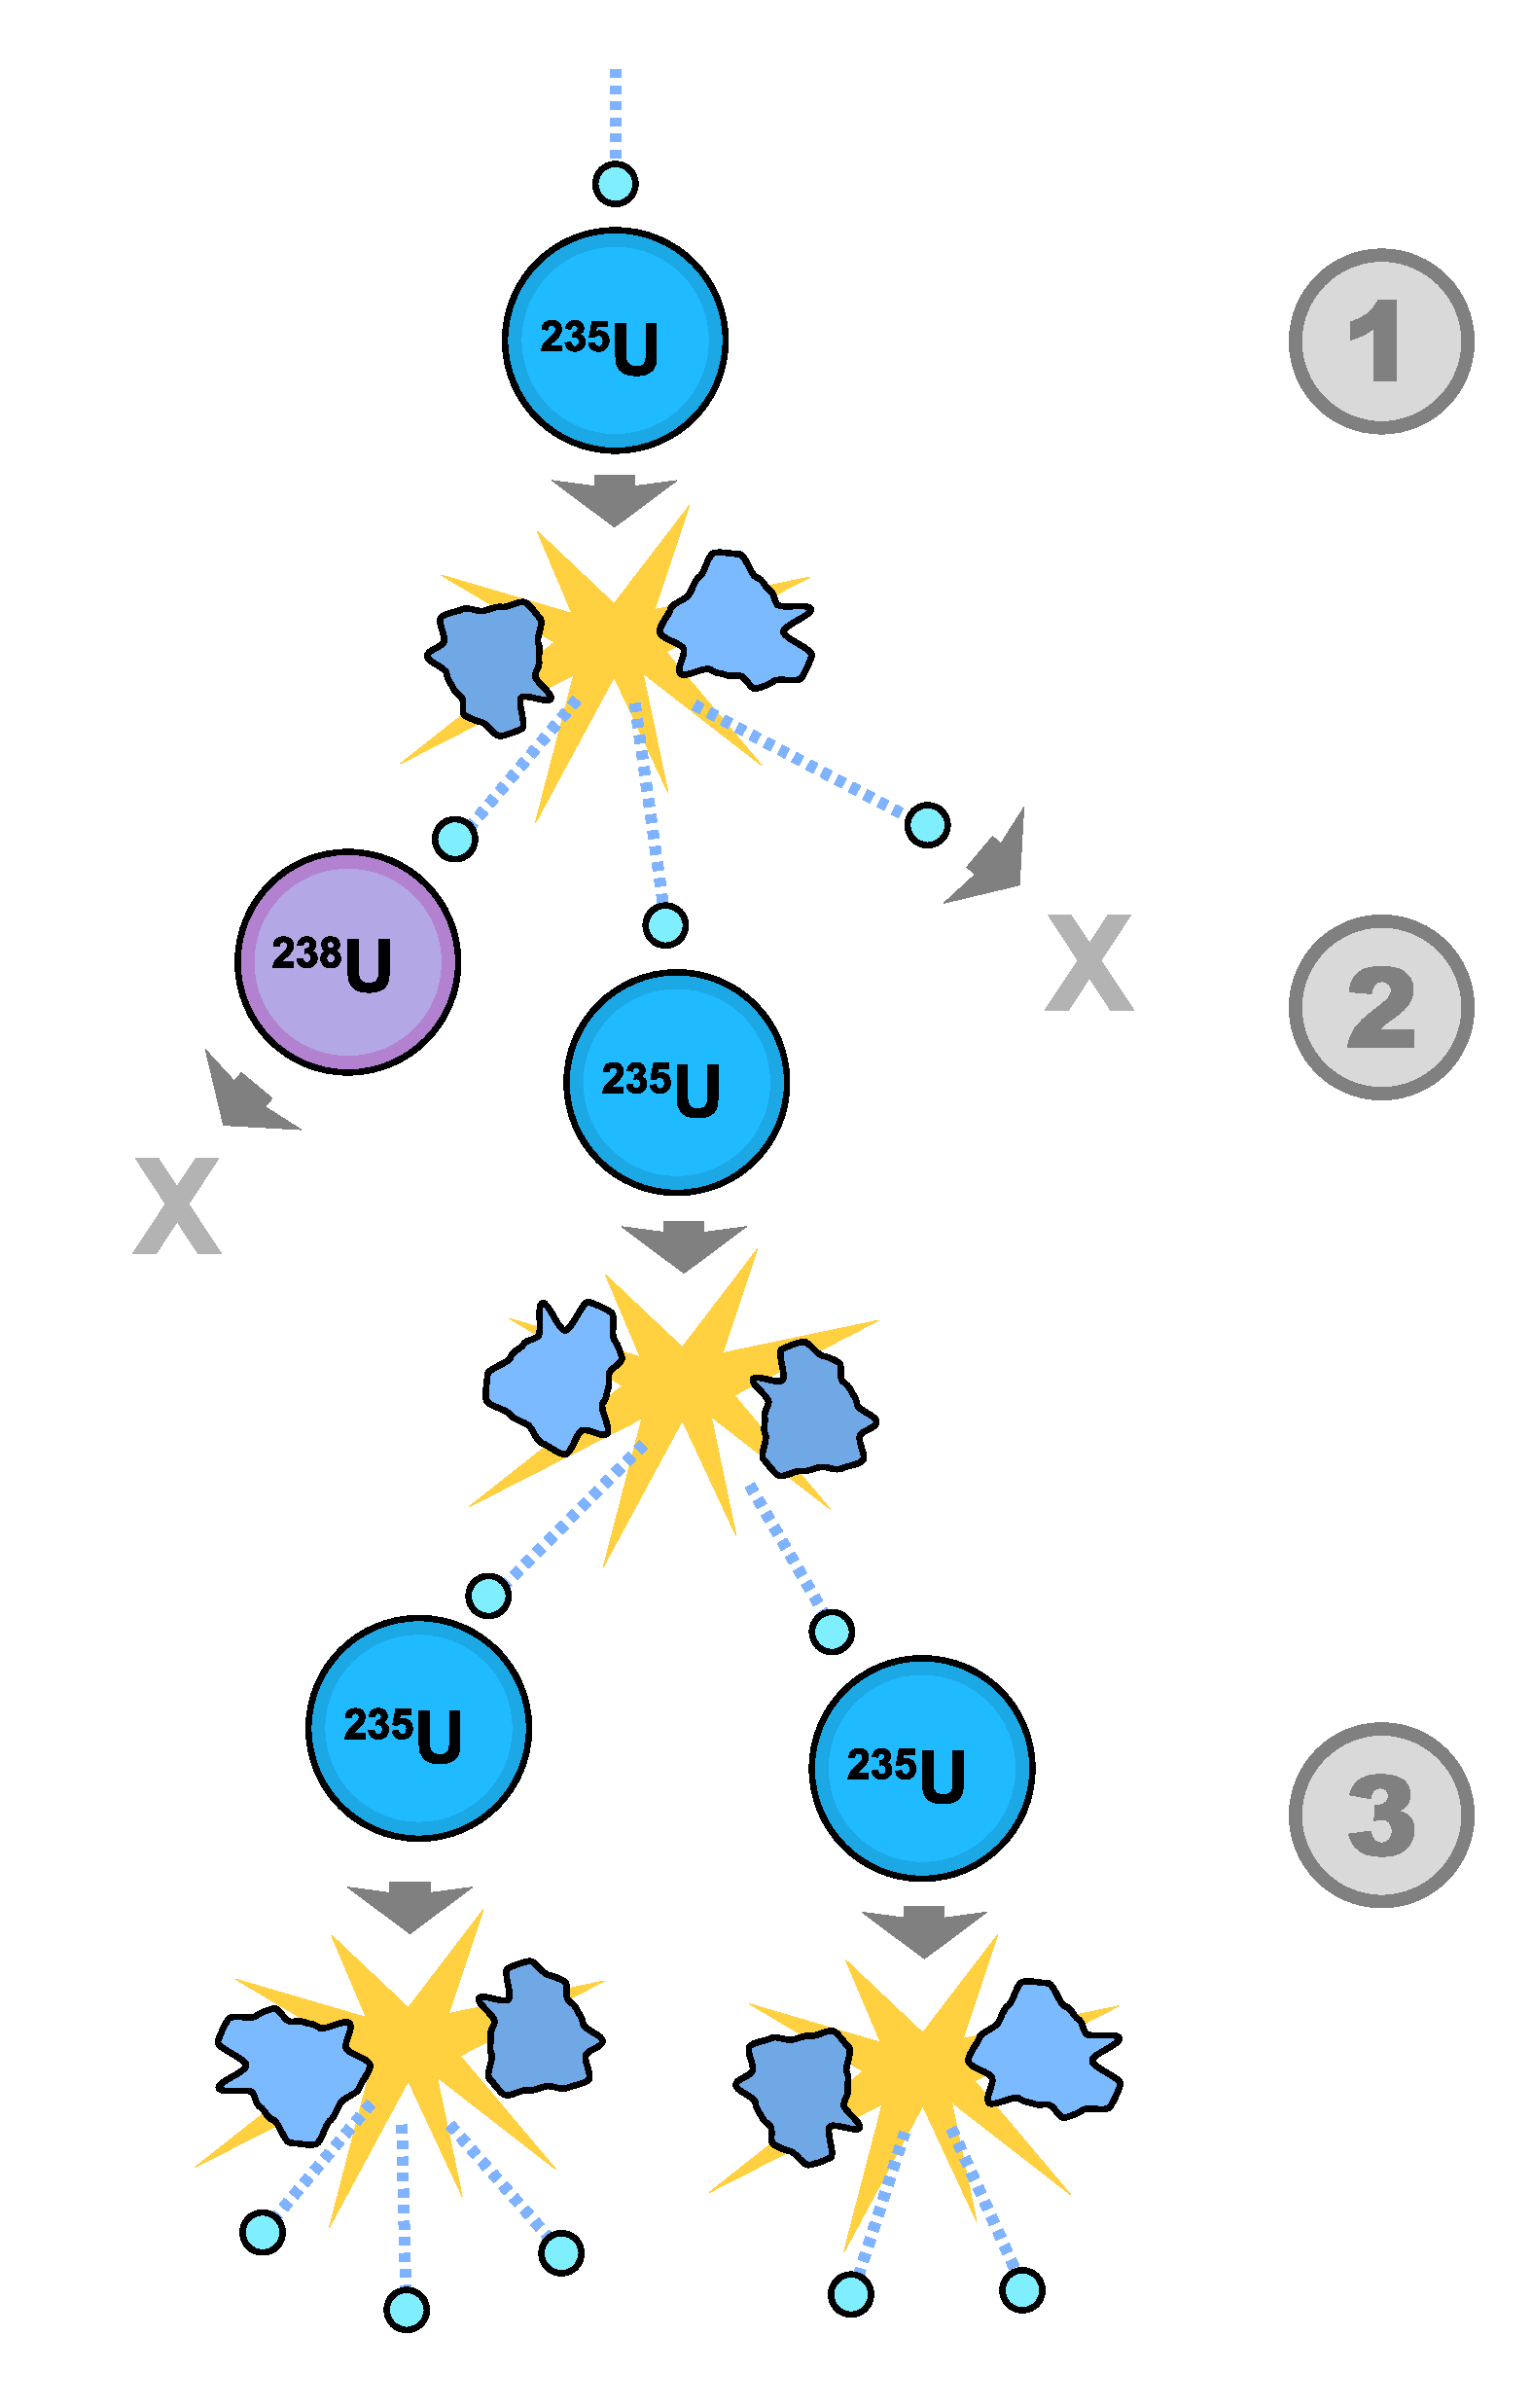
\includegraphics[width=0.7\textwidth]{./img/chainReaction.pdf}
                        \caption*{The fission chain reaction}
                    \end{figure}
                \end{column}

            \end{columns}

        \end{frame}

        \begin{frame}{The US nuclear fleet is composed of \\ roughly 100 light water reactors (LWR)}

            \begin{columns}[T]

                \begin{column}{0.5\textwidth}
                    \begin{figure}
                        \centering
                        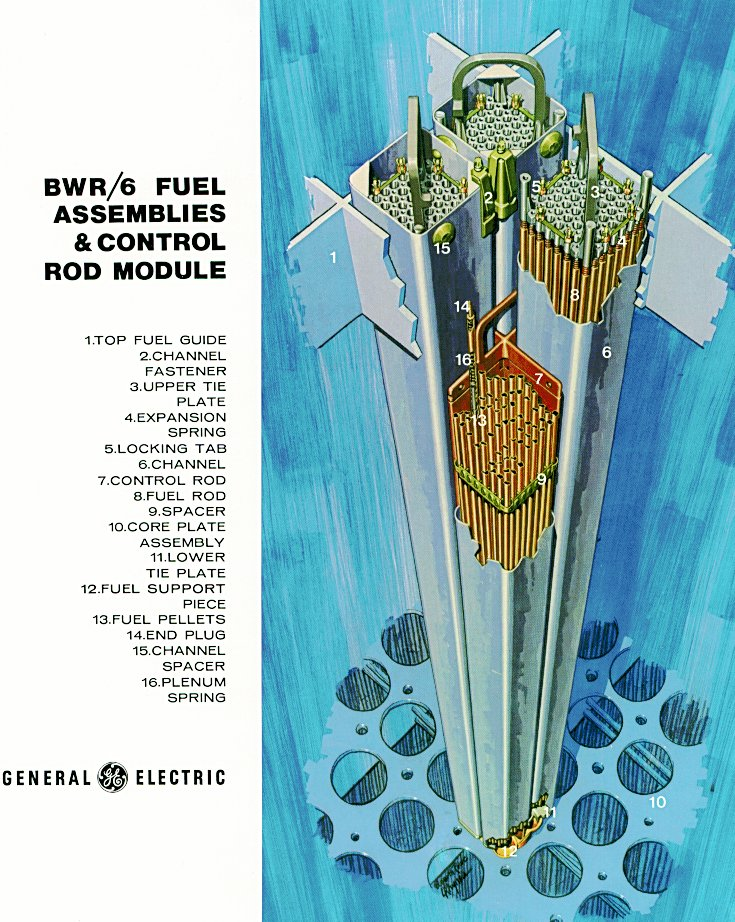
\includegraphics[width=0.8\textwidth]{./img/bwrFuel.png}
                        \caption*{A fuel assembly}
                    \end{figure}
                \end{column}

                \begin{column}{0.5\textwidth}
                    \begin{figure}
                        \centering
                        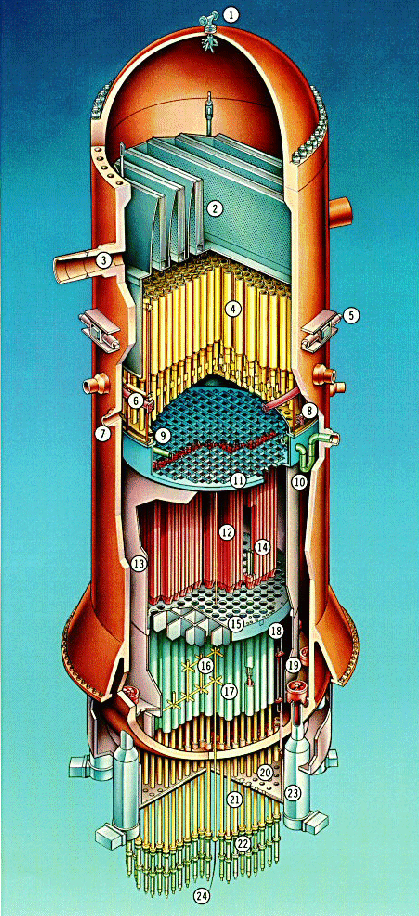
\includegraphics[width=0.5\textwidth]{./img/bwrCore.png}
                        \caption*{A nuclear reactor core}
                    \end{figure}
                \end{column}

            \end{columns}

        \end{frame}

        \begin{frame}{Nuclear reactors power 1800's era steam engines \\ just like coal, oil, and some natural gas}

            \begin{columns}[T]

                \begin{column}{0.5\textwidth}
                    \begin{figure}
                        \centering
                        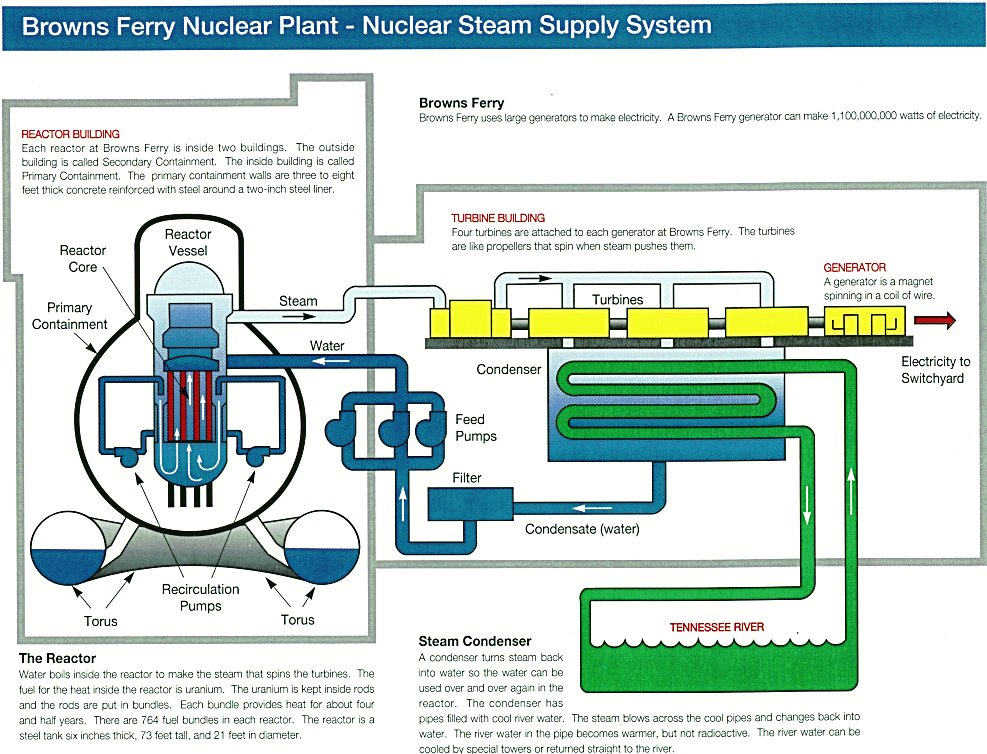
\includegraphics[width=\textwidth]{./img/bwrBop.png}
                        \caption*{Neutrons to electrons}
                    \end{figure}
                \end{column}

                \begin{column}{0.5\textwidth}
                    \begin{itemize}
                        \item Fission chain reaction releases heat
                        \pause
                        \item ... which boils water
                        \pause
                        \item ... which turns a turbine
                        \pause
                        \item ... which rotates a generator
                        \pause
                        \item ... which generates electricity!
                        \pause

                        \vspace{2em}

                        \item One third of heat energy is converted to electricity

                    \end{itemize}
                \end{column}

            \end{columns}

        \end{frame}

        \begin{frame}{There is room for improvement}
            \begin{itemize}
                \item Spent nuclear fuel is waiting for disposal
                \pause
                \item The core needs to be actively cooled
                \pause
                \item The fuel can melt
                \pause
                \item The water must be at high pressures
                \pause
                \item Two-thirds of energy is lost
            \end{itemize}
        \end{frame}

        \begin{frame}{We have come a long way since 1978}
            \begin{itemize}
                \item The most recent plant was built in 1996
                \pause
                \item ... its construction began in 1978
                \pause
                \item ... its design process took place in the early 1970's
                \pause
                \item We can do better!
            \end{itemize}
        \end{frame}

    \subsection{... is new}

        \begin{frame}{Sodium-cooled Fast reactors (SFR) consume nuclear waste, recycle it, and consume it again}
            \begin{figure}
                \centering
                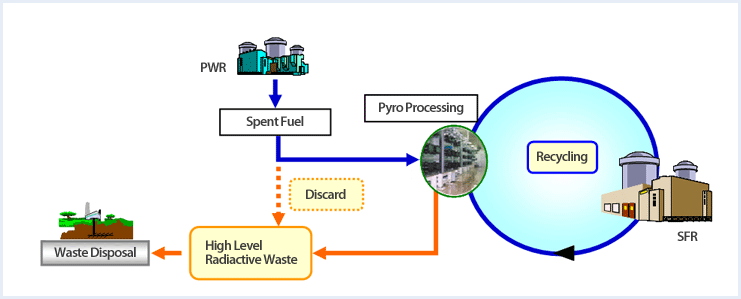
\includegraphics[width=1.0\textwidth]{./img/fastCycle.png}
                \caption*{}
            \end{figure}
        \end{frame}

        \begin{frame}{Traveling wave reactors (TWR; Breed \& Burn reactors) breed their own fuel without reprocessing}
            \begin{figure}
                \centering
                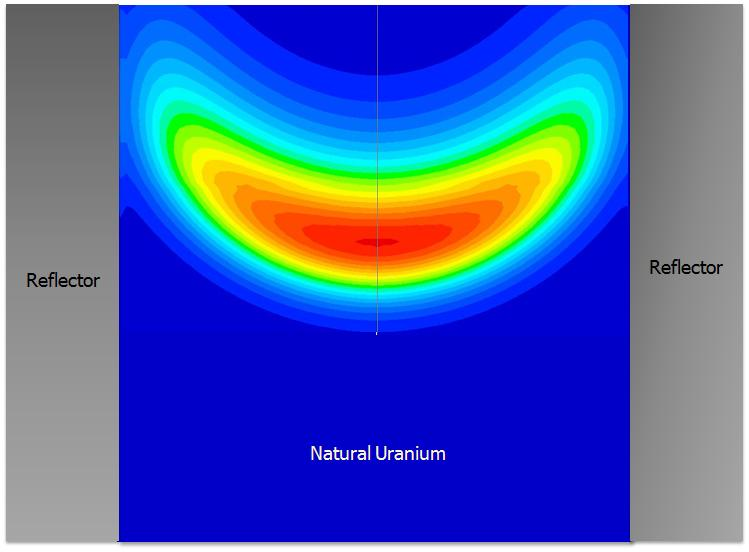
\includegraphics[width=0.9\textwidth]{./img/candle.png}
                \caption*{}
            \end{figure}
        \end{frame}

        \begin{frame}{Fluoride-salt high-temperature reactors (FHR) \\ can be passively cooled with ambient air}
            \begin{figure}
                \centering
                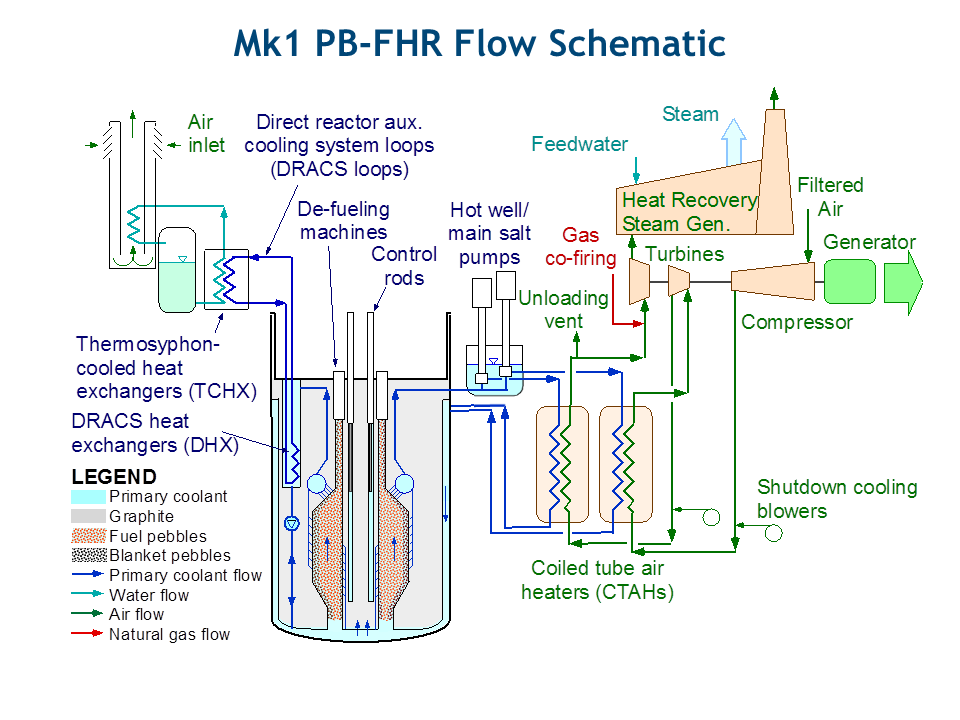
\includegraphics[width=0.9\textwidth]{./img/fhrBop.png}
                \caption*{}
            \end{figure}
        \end{frame}

        \begin{frame}{FHR's use coated particle fuel which cannot melt}
            \begin{figure}
                \centering
                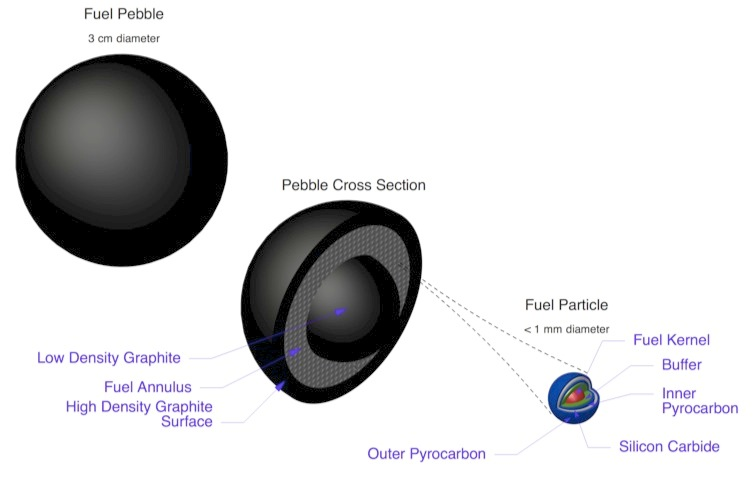
\includegraphics[width=1.0\textwidth]{./img/fhrPebble.png}
                \caption*{}
            \end{figure}
        \end{frame}

        \begin{frame}{FHR's replace water with fluoride salts \\ which boil at 1430$^{\circ}$C}
            \begin{figure}
                \centering
                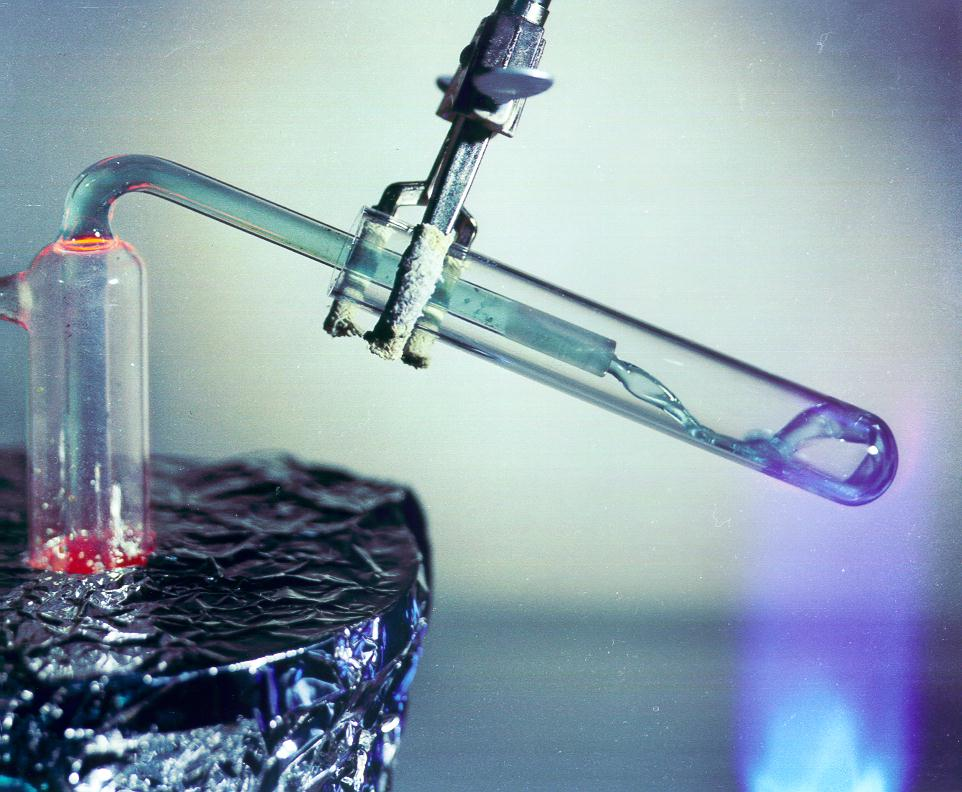
\includegraphics[width=0.8\textwidth]{./img/fhrFlibe.png}
                \caption*{}
            \end{figure}
        \end{frame}

        \begin{frame}{FHR's use modern air turbines \\ which are efficient and offer load following}
            \begin{figure}
                \centering
                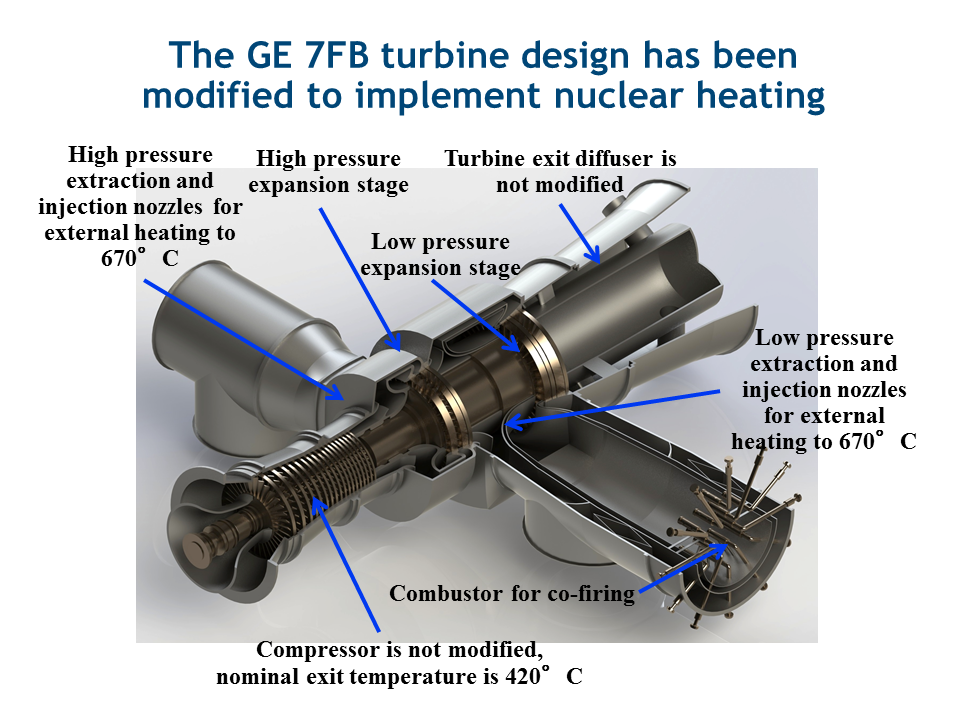
\includegraphics[width=0.9\textwidth]{./img/fhrPower.png}
                \caption*{}
            \end{figure}
        \end{frame}

        FIXME

        \begin{frame}{Hybrid fusion-fission reactors}{... still need some work}
            \begin{figure}
                \centering
                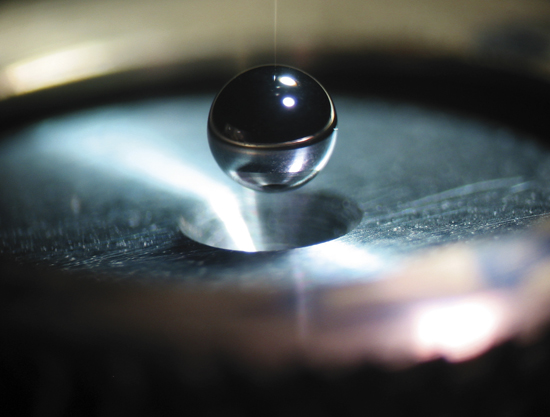
\includegraphics[width=0.9\textwidth]{./img/lifeFuel.png}
                \caption*{}
            \end{figure}
        \end{frame}

        \begin{frame}{Hybrid fusion-fission reactors}{.. are envisioned as a stepping-stone between fission and fusion energy}
            \begin{figure}
                \centering
                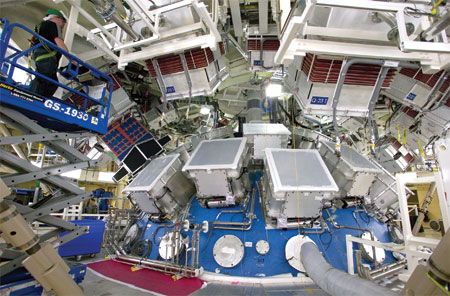
\includegraphics[width=1.0\textwidth]{./img/nifChamber.png}
                \caption*{}
            \end{figure}
        \end{frame}

        \begin{frame}{Hybrid fusion-fission reactors}{.. are awesome}
            \begin{figure}
                \centering
                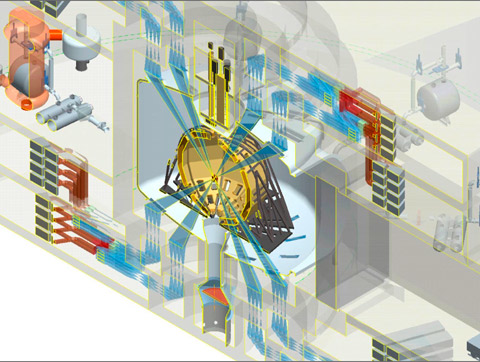
\includegraphics[width=0.9\textwidth]{./img/lifeChamber.png}
                \caption*{}
            \end{figure}
        \end{frame}

\section{Simulations}

    \subsection{The neutron transport equation}

        \begin{frame}{Accurate simulation of neutron fields requires their description 7-dimensional neutron phase space}
            \begin{figure}
                \centering
                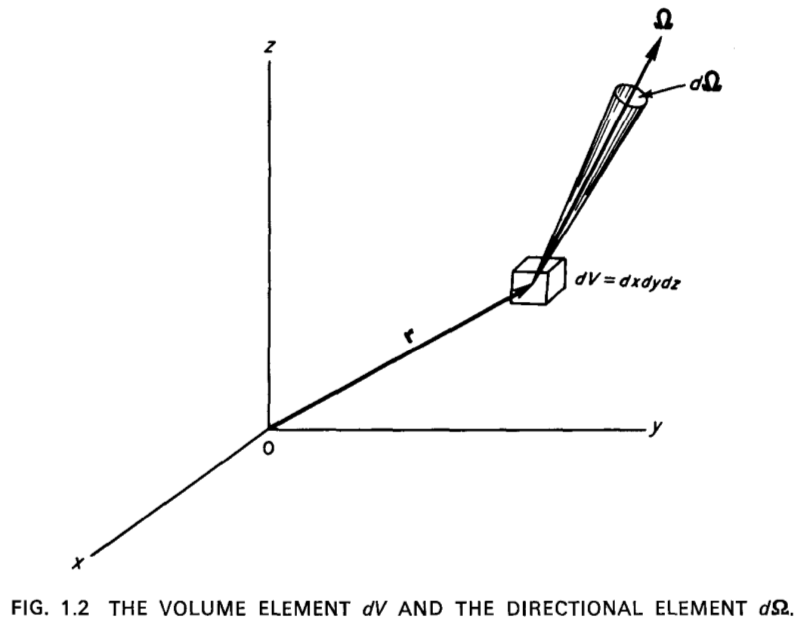
\includegraphics[width=0.9\textwidth]{./img/phaseSpace.png}
            \end{figure}
        \end{frame}

        \begin{frame}{Spatial distributions $(\vec r)$ can be complicated}
            \begin{figure}
                \centering
                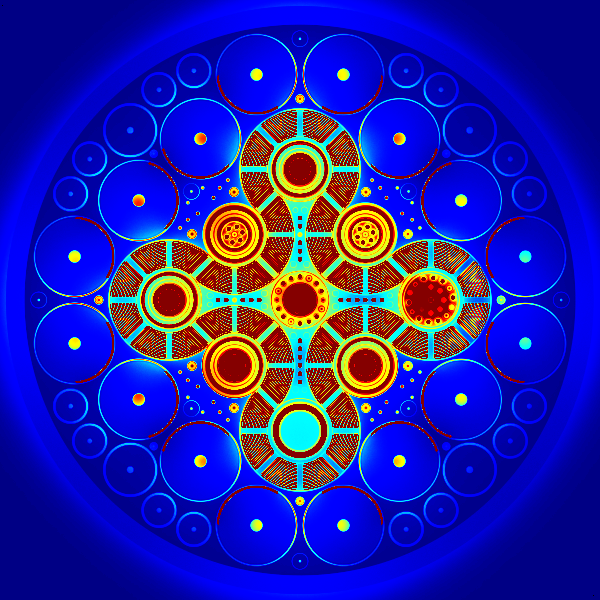
\includegraphics[width=0.7\textwidth]{./img/spaceFlux1.png}
                \caption*{}
            \end{figure}
        \end{frame}

        \begin{frame}{Spatial distributions $(\vec r)$ can be complicated}
            \begin{figure}
                \centering
                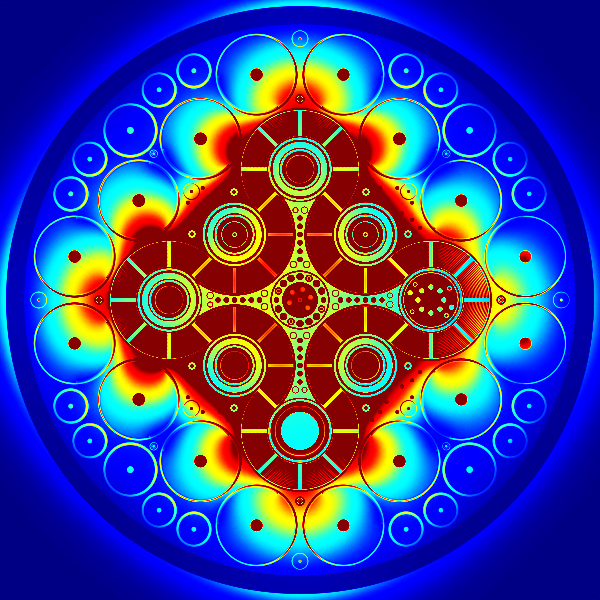
\includegraphics[width=0.7\textwidth]{./img/spaceFlux2.png}
                \caption*{}
            \end{figure}
        \end{frame}

        \begin{frame}{Spatial distributions $(\vec r)$ can be complicated}
            \begin{figure}
                \centering
                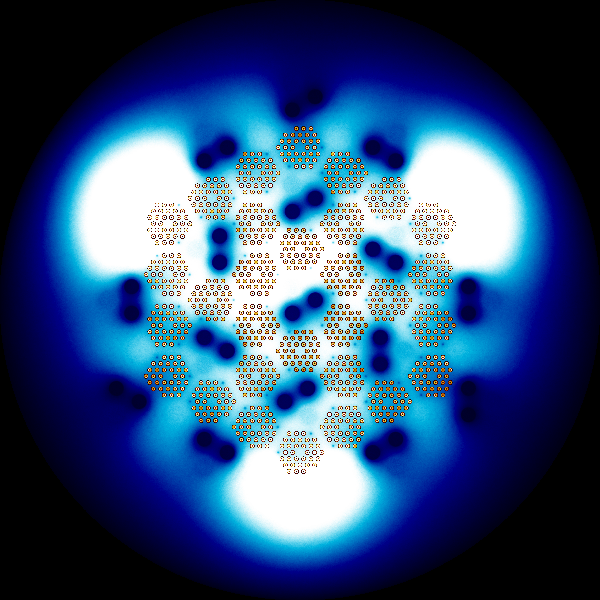
\includegraphics[width=0.7\textwidth]{./img/spaceFlux3.png}
                \caption*{}
            \end{figure}
        \end{frame}

        \begin{frame}{Energy distributions $(E)$ can be complicated}
            \begin{figure}
                \centering
                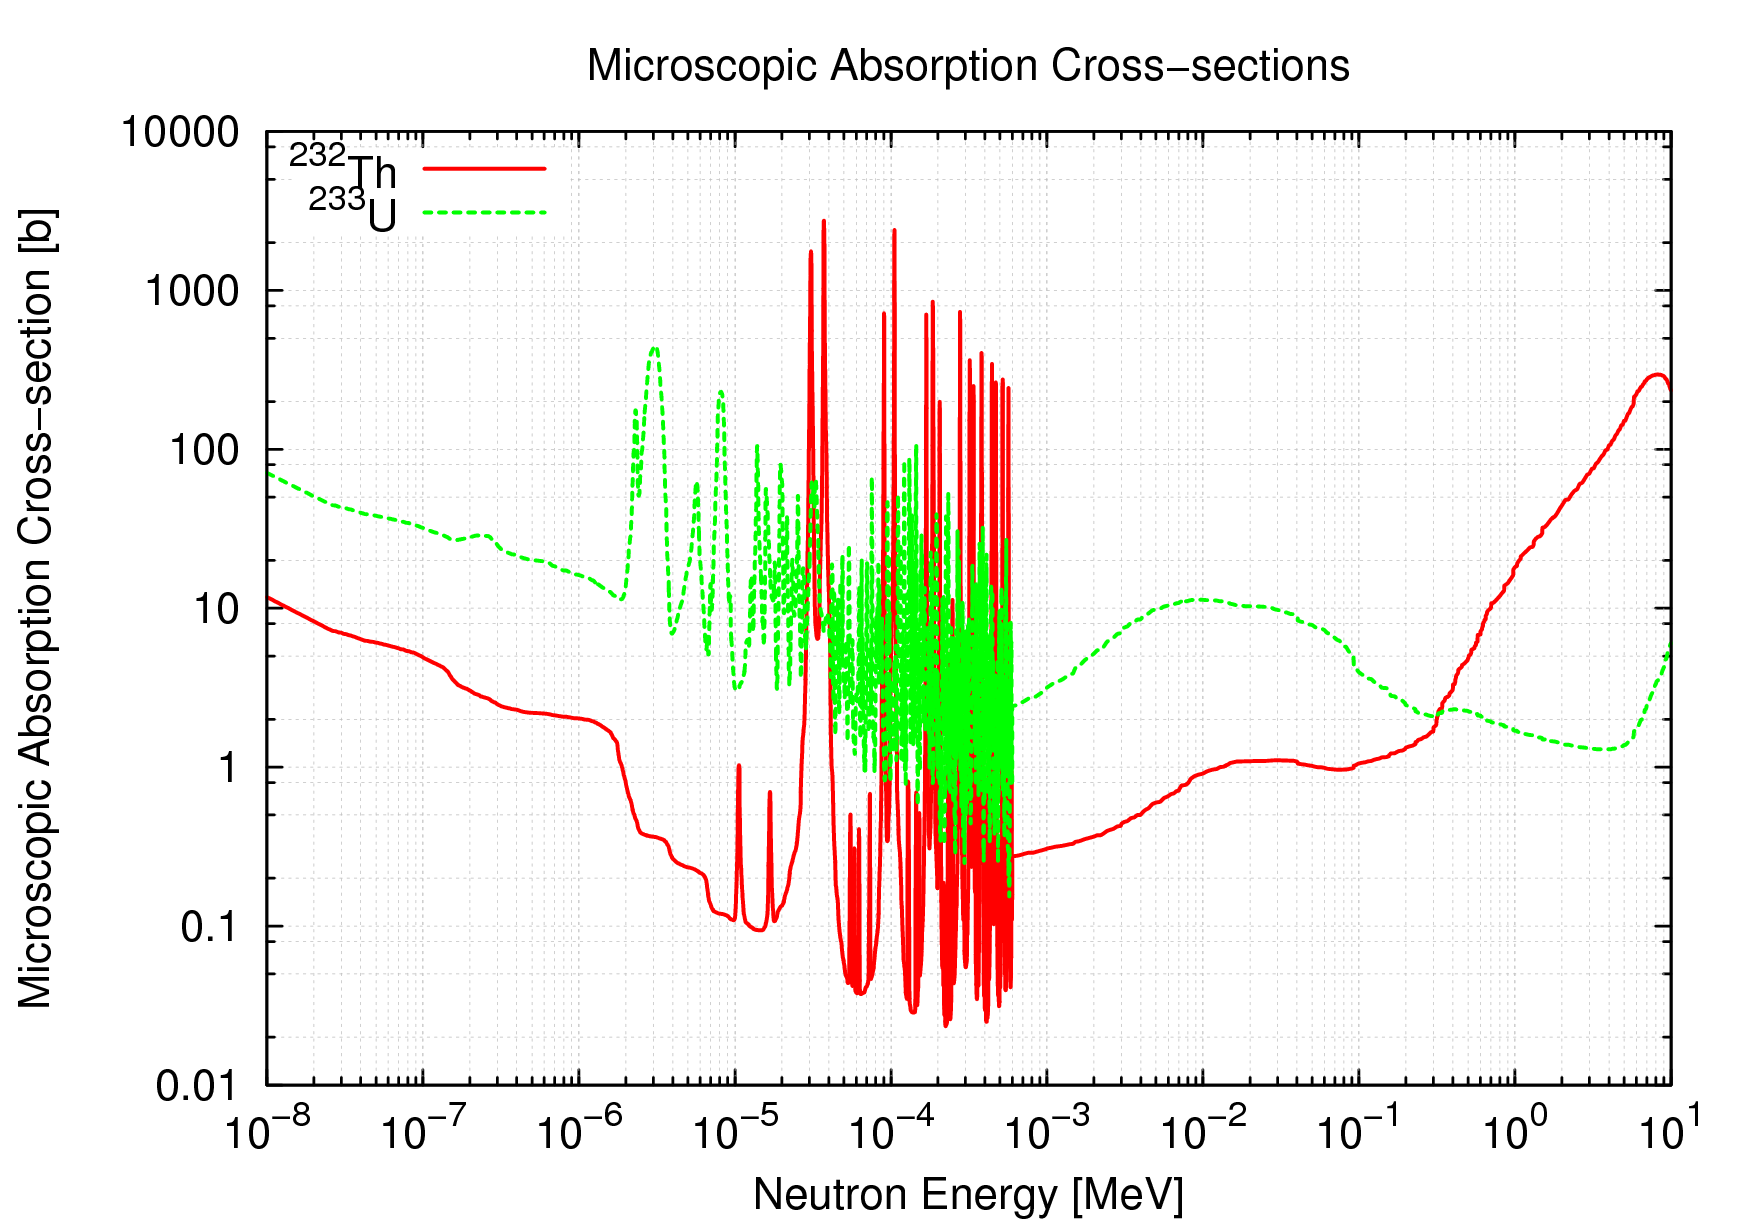
\includegraphics[width=1.0\textwidth]{./img/energyXs.png}
                \caption*{}
            \end{figure}
        \end{frame}

        \begin{frame}{Energy distributions $(E)$ can be complicated}
            \begin{figure}
                \centering
                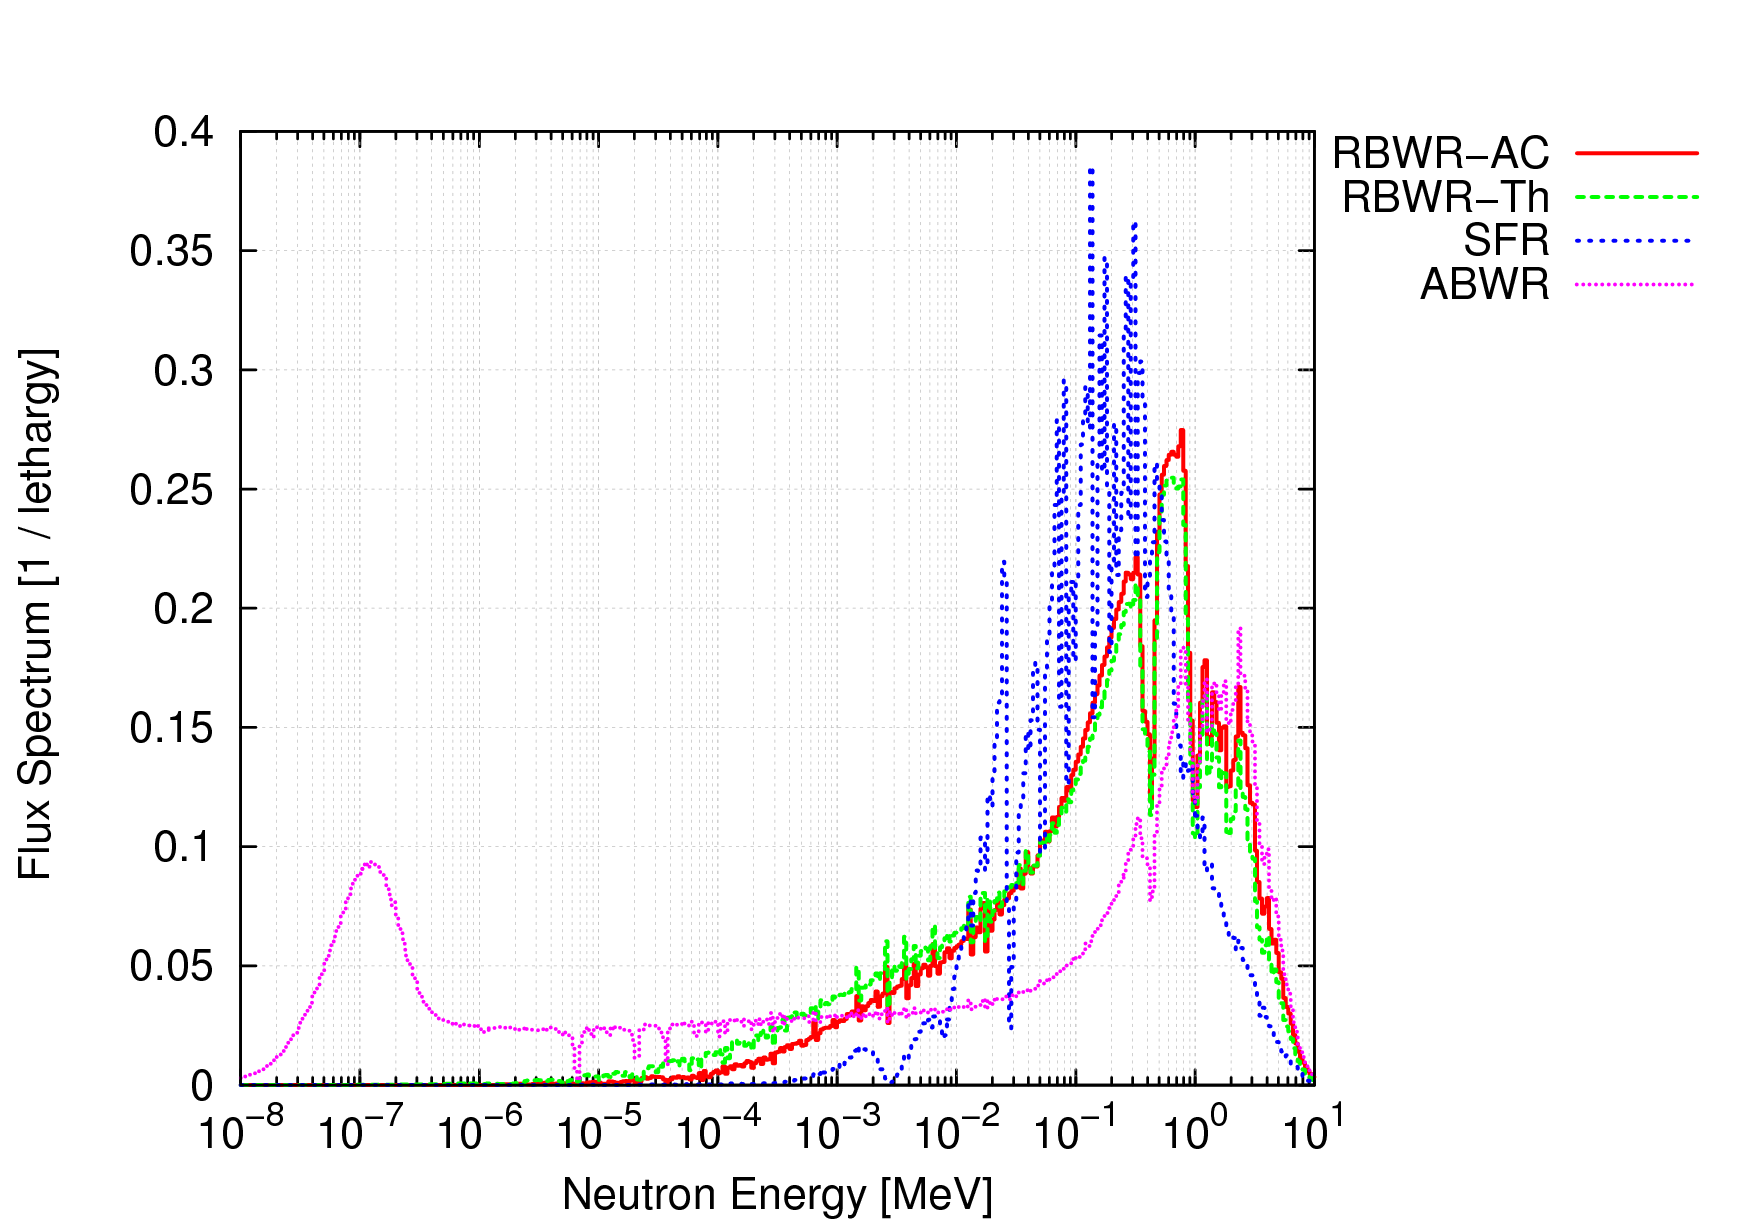
\includegraphics[width=1.0\textwidth]{./img/energyFlux.png}
                \caption*{}
            \end{figure}
        \end{frame}

        \begin{frame}{The neutron transport equation balances sources and sinks within this neutron phase space}{(time dependence is omitted for simplicity)}
            \begin{equation*}
                \begin{split}
                    \vec \Omega \cdot \vec \bigtriangledown \; \; \psi(\vec r, E, \vec \Omega) \\
                    + \sigma_{total}(\vec r, E) \; \; N(\vec r) \; \; \psi(\vec r, E, \vec\Omega) \\
                    = \int_0^\infty \! \! \! \! dE \int_{4\pi} \! \! \! \! d\vec\Omega \; \; \sigma_{scatter}(\vec r, E^\prime \rightarrow E, \vec \Omega^\prime \cdot \vec \Omega) \; \; N(\vec r) \; \; \psi(\vec r, E^\prime, \vec\Omega^\prime) \\
                    + \frac{\chi(E)}{4\pi} \int_0^\infty \! \! \! \! dE^{\prime\prime} \; \; \nu (E^{\prime\prime}) \; \; \sigma_{fission}(\vec r, E^{\prime\prime}) \; \; N(\vec r) \; \; \psi(\vec r, E^{\prime\prime}, \vec\Omega^{\prime\prime}) \\
                    + \mathcal{S}_{ext}(\vec r, E, \vec\Omega)
                \end{split}
            \end{equation*}
        \end{frame}

        \begin{frame}{Simplification, Discretization, Monte Carlo}
        \end{frame}

        \begin{frame}{Coupled simulations}
        \end{frame}

    \subsection{The Bateman equations}

        \begin{frame}{Isotope depletion, breeding, and decay $(t)$ can be complicated}
            \begin{figure}
                \centering
                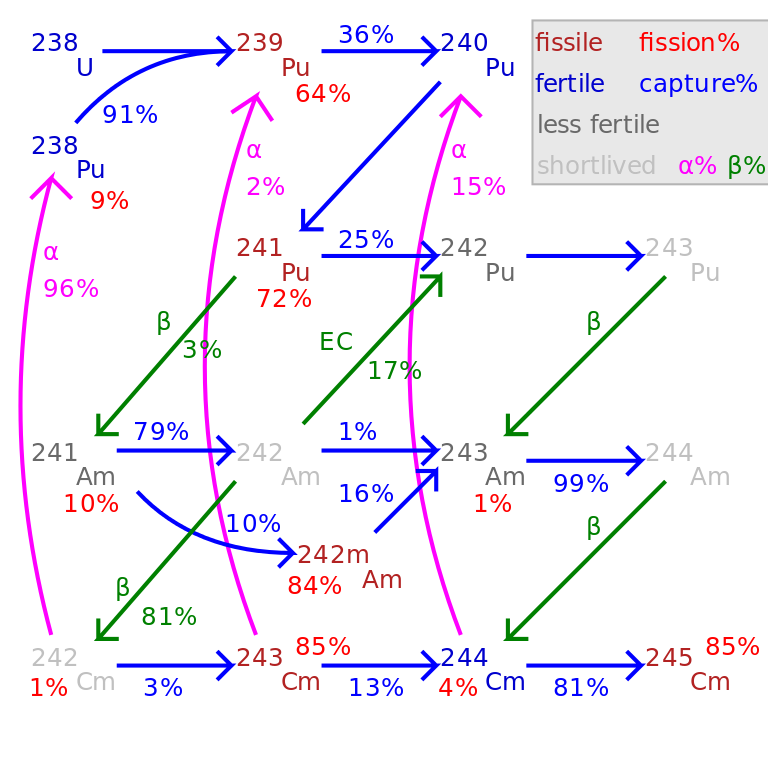
\includegraphics[width=0.7\textwidth]{./img/fuelCycle.png}
                \caption*{}
            \end{figure}
        \end{frame}

        \begin{frame}{The Bateman equations describe the time-evolution of isotopes during decay and irradiation}{... it must be solved simultaneously with the NTE}
            \begin{equation*}
                \begin{split}
                    \frac{\partial N_i(\vec r, t)}{\partial t} \\
                    + \lambda_i \; \; N_i(\vec r, t) \\
                    + \int_0^\infty \! \! \! \! dE \; \; \sigma_{absorption,i} ( \vec r, E) \; \; \int_{4\pi} \! \! \! \! d\vec\Omega \; \; \psi(\vec r, E, \vec \Omega) \; \; N_i(\vec r, t) \\
                    = \sum_j \left[ b_{j \rightarrow i} \; \; \lambda_j \; \; N_j(\vec r, t) \right] \\
                    + \sum_k \left[ b_{k \rightarrow i} \int_0^\infty \! \! \! \! dE \; \; \sigma_{absorption,k} ( \vec r, E) \; \; \int_{4\pi} \! \! \! \! d\vec\Omega \; \; \psi(\vec r, E, \vec \Omega) \; \; N_k(\vec r, t) \right] \\
                \end{split}
            \end{equation*}
        \end{frame}

        \begin{frame}{Analytical, Matrix Exponential, CRAM}
        \end{frame}

\section*{Summary}

    \begin{frame}{Summary}
    \end{frame}

\end{document}
